% This document should describe the entire assembly of the device, NOTE: only some devices will be pre-soldered so include some form of table of contents to jump to if you're buoy is pre-soldered.
\section{Device Construction}

\subsection{Production Buoy}

\subsection{Prototype Buoy}

\begin{flushleft}
    The prototype instructions are to set up the user with a breadboard layout of the buoy in order to have a more 
    accessible format of making changes and updates to the design of the hardware buoy.
\end{flushleft}

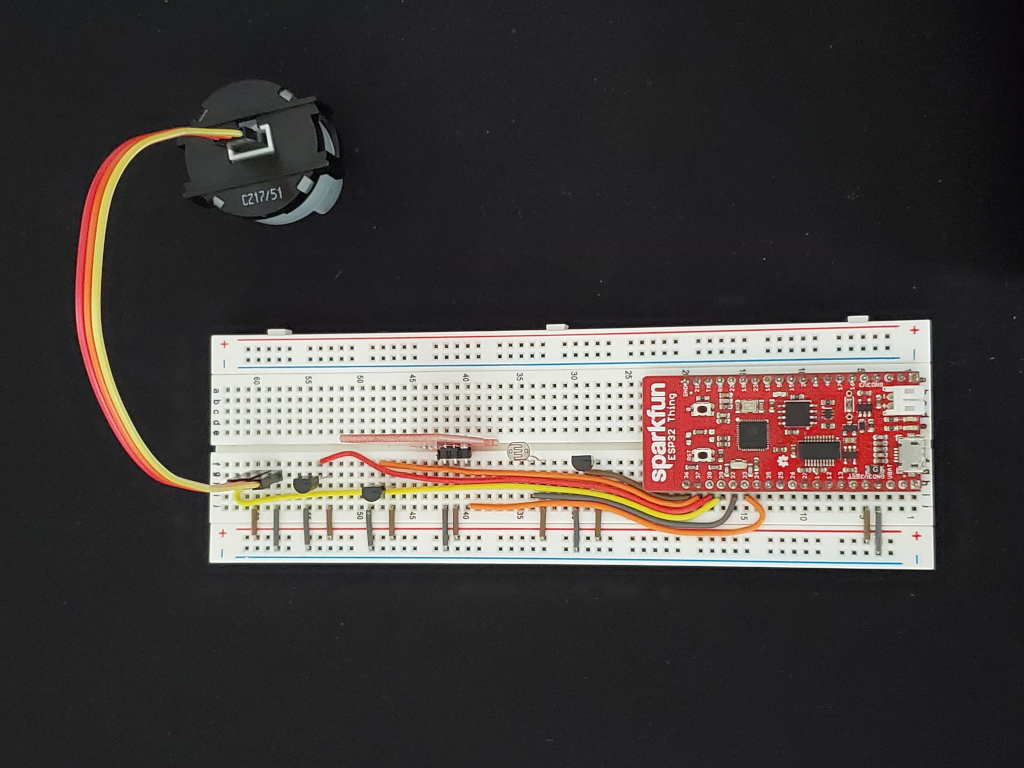
\includegraphics[scale=1]{buoy_breadboard.jpg}

\begin{enumerate}
    \item Place the Sparkfun ESP32 on the end of the breadboard and offset right from the center of the breadboard,
    so the left-side GPIO pins have more room to insert jumper wires. The pins on the Sparkfun should go in \textbf{Columns 1 through 20}, for the \textbf{Rows A and H}.
    \item Insert the jumper wires for the breadboard power rails, connecting the ESP32 pin \textbf{3V3} to the Positive rail and ESP32 pin \textbf{GND} to the Negative rail.
    \item Add the first temprature sensor to \textbf{Columns 28, 29, 30}, flat-side facing to the middle of the breadboard. Connect \textbf{Column 28 to Positive Rail} and \textbf{Column 30 to Negative Rail}. Connect \textbf{Column 29 to Column 20} which connects to ESP32 pin \textbf{36}.
    \item Add the photoresistor to \textbf{Columns 33, 34}, polarity does not matter. Connect \textbf{Column 33 to Positive Rail} and \textbf{Column 34 to Column 16} which connects ESP32 pin \textbf{32}.
    \item Add the salinty sensor to \textbf{Columns 40, 41, 42}, Power LED facing away from center of breadboard. Connect \textbf{Column 42 to Negative Rail}, \textbf{Column 41 to Positive Rail}, and \textbf{Column 40 to Column 15} which is ESP32 pin \textbf{33}.
    \item Add the second temprature sensor to \textbf{Columns 47, 48, 49}, flat-side facing to the middle of the breadboard. Connect \textbf{Column 47 to Positive Rail} and \textbf{Column 49 to Negative Rail}. Connect \textbf{Column 48 to Column 20} which connects to ESP32 pin \textbf{37}.
    \item Add the third temprature sensor to \textbf{Columns 53, 54, 55}, flat-side facing to the middle of the breadboard. Connect \textbf{Column 28 to Positive Rail} and \textbf{Column 30 to Negative Rail}. Connect \textbf{Column 29 to Column 20} which connects to ESP32 pin \textbf{38}.
    \item Add the insolation sensor (tab connector orientated up), where the \textbf{Left Pin is +5V}, \textbf{Center Pin is output}, and \textbf{Right Pin is GND} to \textbf{Columns 60, 59 , 58} respectively. Connect \textbf{Column 60 to Positive Rail}, \textbf{Column 58 to Negative Rail}, and \textbf{Column 59 to Column 17} which is ESP32 pin \textbf{39}.
\end{enumerate}